\section{Results}
\label{sec:experiments}


We evaluate \ourmethod, validating that (i) co-evolved learned evaluation improves search even on verifiable coding tasks where ground truth exists, exceeding the \hgmh held-out pass rate at lower search cost~(\cref{sec:exp-polyglot}), and (ii) co-evolution improves generators in domains where no benchmark can score the artifact, yielding stronger paper writers and Olympiad provers~(\cref{sec:exp-writer}). \Cref{sec:analysis} then examines how utility transitions shape the search. We then validate that (iii) co-evolution improves the evaluators themselves, strengthening the grader and correcting the paper reviewer's over-leniency toward \AI-generated text~(\cref{sec:exp-adversarial}). Finally, we provide a targeted ablation showing that lower-cost search-time task-agent calls can preserve paper-domain endpoints when the final scoring model is held fixed~(\cref{sec:reducing_search_costs}). Further details and ablations are in \cref{app:exp-details,app:extended-results}.



\subsection{Learned evaluation helps even where ground truth exists (RQ1)}
\label{sec:exp-polyglot}

We now show \ourmethod improves search even in domains where objective ground-truth evaluation exists. In the \polyglot coding domain, we co-evolve a code reviewer alongside the coder. Because \polyglot is built around multi-turn agent editing, this agent-as-a-judge provides a much cheaper and complementary surrogate objective. The meta-agent learns not just whether a patch passes tests, but also whether it is of high quality. \Theourmethod exceeds the \hgmh held-out pass rate for both the specialist and generalist at $1.35\times$--$1.72\times$ lower token cost~(\cref{fig:intro-token-efficiency}). Examining where the meta-agent edits the codebase shows why co-evolving the two roles pays off: in the \polyglot run, $90\%$ of accepted patches modify shared task-agent functionality or infrastructure used by both the coder and the reviewer, rather than role-specific code~(\cref{fig:analysis-transfer}). A single such edit therefore improves both roles, suggesting co-evolution enriches the search rather than splitting effort across competing objectives.

\takeawaybox[RQ1:]{\ourmethod is a general framework for enriching the utility signals available to a search: even where ground truth exists, co-evolving a learned evaluator supplies a complementary objective that improves search efficiency, with promise for domains where evaluation is even slower.}


\subsection{Learned evaluation improves agents on domains without objective evaluation~(RQ2)}
\label{sec:exp-writer}






We now turn to domains with no objective benchmark, where only evaluator-dependent task agents exist. We score the artifacts produced by our paper writer and prover against a broad panel of reviewers and graders from both our work and prior baselines. The task agents and their evaluators interact throughout the search, but in this section we evaluate only the task agents, deferring evaluators to \cref{sec:exp-adversarial}, where objective anchor data permits further analysis.



\noindent\textbf{Paper writing.}~~Paper quality cannot be evaluated objectively, so we score writer artifacts against a fixed panel of four reviewers from our work and prior baselines~(\cref{tab:paper-writer-cross-reviewer}); the joint search of the writer and its co-evolving reviewer is shown on the right in \cref{fig:paper-writer-reviewer-results}. Our results show that co-evolving the writer with a learned reviewer improves it. At the matched-compute point where \hgmh commits to its writer, our writer already achieves a $1.78\times$ higher reviewer-panel acceptance rate on average, and across the full run it beats \hgmh as evaluated by every reviewer, with a $1.86\times$ higher acceptance rate. This is enabled by a co-evolving reviewer whose objective is regularized to favor reviewers harsher on \AI-generated text~(\cref{sec:exp-adversarial}), giving the writer a stricter signal resilient to reward hacking.


\begin{table}[htbp]
\centering
\caption{\textbf{Co-evolved writers achieve $1.78\times$ higher mean acceptance than \hgmh at matched search cost, and $1.86\times$ for the best-found specialist.} Rows are writer agents; the four \textbf{Reviewers} columns form a fixed panel from our work and prior baselines, each cell giving the percentage of writer-generated papers that reviewer accepts (mean $\pm$ 95\% Jeffreys interval). \textbf{Mean} averages across the panel, with each \ourmethod writer's gain over \hgmh in parentheses. \textbf{\ourmethod adversarial} is the \ourmethod reviewer regularized to be harsher on \AI-written text (\cref{sec:exp-adversarial}). Best per column in \textbf{bold}.}
\label{tab:paper-writer-cross-reviewer}
\small
\setlength{\tabcolsep}{5.0pt}
\renewcommand{\arraystretch}{1.12}
\begin{tabular}{lrcccc@{\hskip 10pt}r}
\toprule
& & \multicolumn{4}{c}{\textbf{Reviewer Acceptance Rate~(\%,~$\uparrow$)}} & \\
\cmidrule(lr){3-6}
\textbf{Writer} & \shortstack[r]{\textbf{Search}\\\textbf{Tokens}} & \shortstack{\textbf{\sakana}\\\textbf{\citep{lu2024ai}}} & \shortstack{\textbf{\dgmh}\\\textbf{\citep{zhang2026hyperagents}}} & \shortstack{\textbf{\hgmh}\\\textbf{\citep{wang2025huxley,zhang2026hyperagents}}} & \shortstack{\textbf{\ourmethod}\\\textbf{adversarial}} & \makebox[6.8em][c]{\textbf{Mean~(\%,~$\uparrow$)}} \\
\midrule
\hgmh writer & 42.5M & $1.0$\,{\color{black!55}\scriptsize$\pm 2.2$} & $12.0$\,{\color{black!55}\scriptsize$\pm 6.3$} & $64.0$\,{\color{black!55}\scriptsize$\pm 9.3$} & $10.0$\,{\color{black!55}\scriptsize$\pm 5.9$} & \makebox[6.8em][l]{\makebox[2.5em][r]{$21.8$}\,{\color{black!55}\scriptsize$\pm 4.0$}\,\makebox[2.6em][l]{}} \\
\addlinespace[2pt]
\ourmethod writer (generalist) & 44.6M & $2.0$\,{\color{black!55}\scriptsize$\pm 2.9$} & \textbf{43.0}\,{\color{black!55}\scriptsize$\pm 9.6$} & $81.0$\,{\color{black!55}\scriptsize$\pm 7.6$} & $29.0$\,{\color{black!55}\scriptsize$\pm 8.8$} & \makebox[6.8em][l]{\makebox[2.5em][r]{$38.8$}\,{\color{black!55}\scriptsize$\pm 4.8$}\,\makebox[2.6em][l]{\scriptsize($1.78\times$)}} \\
\addlinespace[2pt]
\ourmethod writer (specialist) & 221.8M & \textbf{5.0}\,{\color{black!55}\scriptsize$\pm 4.3$} & $40.0$\,{\color{black!55}\scriptsize$\pm 9.5$} & \textbf{86.0}\,{\color{black!55}\scriptsize$\pm 6.8$} & \textbf{31.0}\,{\color{black!55}\scriptsize$\pm 9.0$} & \makebox[6.8em][l]{\makebox[2.5em][r]{\textbf{40.5}}\,{\color{black!55}\scriptsize$\pm 4.8$}\,\makebox[2.6em][l]{\scriptsize($1.86\times$)}} \\
\bottomrule
\end{tabular}
\end{table}




\noindent\textbf{Proof writing.}~~The proof domain is substantially harder than paper writing, with improvements emerging only at longer training horizons. As shown in \cref{tab:imo-proof-cross-grader}, \theourmethod generalist performs similarly to \hgmh at matched compute. The divergence appears at longer horizons: \hgmh stagnates, which we posit is because a frozen evaluator eventually ceases to provide an informative signal. The specialist prover that \ourmethod discovers has the best panel-mean score and \texttt{Pass@6} score. As we show in \cref{sec:exp-adversarial}, this is enabled by a co-evolved grader that exceeds \proofautograder and \hgmh, providing evaluations that guide the search toward better solutions than \hgmh can.



A more nuanced comparison is the \imocode baseline of \citet{huang2025winninggoldimo2025}, a human-engineered verification-and-refinement pipeline that achieved gold-medal performance at IMO 2025. \Theourmethod specialist attains a higher panel-mean score and \texttt{Pass@6} rate, but earns them by finding more near-complete proofs ($6$ of $7$), conceding ground on the stricter \texttt{Pass@7} metric. It still exceeds the best \hgmh prover on \texttt{Pass@7}, and already beats the mean score of the \imocode baseline despite using no hand-engineered Olympiad-specific scaffold. Thus, we posit that closing the remaining \texttt{Pass@7} gap depends on increasing the search budget. Details in \cref{app:extended-results}.



\begin{table}[h]
\centering
\caption{\textbf{The co-evolved \ourmethod specialist prover attains the best mean score, while the \hgmh prover and the \ourmethod generalist fall below the baseline.} Rows are prover agents. A fixed panel of three graders from our work and prior baselines scores every prover's proofs, mirroring the reviewer panel of \cref{tab:paper-writer-cross-reviewer}. Because graders report several metrics, we pool each metric across graders, with per-grader results in \cref{tab:proof-per-grader}. \textbf{Score} is the mean grade ($0$--$7$), \textbf{\texttt{Pass@6}} the fraction scoring at least $6$ of $7$, and \textbf{\texttt{Pass@7}} the fraction earning full credit; all report $\pm$ s.e.m. Best per column in \textbf{bold}.}
\label{tab:imo-proof-cross-grader}
\small
\setlength{\tabcolsep}{6.0pt}
\renewcommand{\arraystretch}{1.12}
\begin{tabular}{lrccc}
\toprule
\textbf{Prover} & \textbf{Search Tokens} & \textbf{Score~($\uparrow$)} & \textbf{\texttt{Pass@6}~($\uparrow$)} & \textbf{\texttt{Pass@7}~($\uparrow$)} \\
\midrule
Static \imocode prover & N/A & $4.07$\,{\color{black!55}\scriptsize$\pm 0.42$} & $55.0\%$\,{\color{black!55}\scriptsize$\pm 6.4$} & \textbf{55.0\%}\,{\color{black!55}\scriptsize$\pm 6.4$} \\
\hgmh prover & 21.5M & $3.73$\,{\color{black!55}\scriptsize$\pm 0.43$} & $51.7\%$\,{\color{black!55}\scriptsize$\pm 6.5$} & $45.0\%$\,{\color{black!55}\scriptsize$\pm 6.4$} \\
\ourmethod prover (generalist) & 37.9M & $3.73$\,{\color{black!55}\scriptsize$\pm 0.43$} & $51.7\%$\,{\color{black!55}\scriptsize$\pm 6.5$} & $45.0\%$\,{\color{black!55}\scriptsize$\pm 6.4$} \\
\ourmethod prover (specialist) & 88.0M & \textbf{4.33}\,{\color{black!55}\scriptsize$\pm 0.41$} & \textbf{61.7\%}\,{\color{black!55}\scriptsize$\pm 6.3$} & $48.3\%$\,{\color{black!55}\scriptsize$\pm 6.5$} \\
\bottomrule
\end{tabular}
\end{table}


\takeawaybox[RQ2:]{Where no objective benchmark exists, co-evolving agents with learned evaluators outperform fixed-evaluator baselines: writers reach markedly higher reviewer-panel acceptance, while provers improve over longer horizons as the co-evolved grader becomes more accurate and the frozen baseline stagnates.}


\subsection{Evaluator replacements act as a curriculum on the search (RQ3)}
\label{sec:analysis}
\begin{figure}[htbp]
    \centering
    
\includegraphics[width=\linewidth]{figures/fig_transition_rerank.pdf}
   \caption{\textbf{Evaluator replacements permanently re-rank the archive.} Each curve tracks one replacement, plotting the Spearman $\rho$ between post- and pre-replacement rankings as evaluations accumulate: $\rho = 1$ (dotted) is the unchanged order, $\rho = 0$ an uncorrelated reordering. Across all three tasks $\rho$ settles well below $1$ and never recovers, so the new ordering holds. The no-erasure control (rightmost) stays high ($\rho \geq 0.90$), showing erasure is necessary for utility transitions to guide search.}
    \label{fig:transition-rerank}
\end{figure}
A potential mechanism by which \theourmethod can improve task agents is that a progressively stronger evaluator hardens the population over time, imposing a curriculum-like effect on the task agents. For this to hold, each transition must achieve two outcomes at once: re-rank the search under the new, stricter criterion rather than leave the old ordering in place, while still letting a strong lineage carry forward so the population advances over time rather than restarting on every transition.

\noindent\textbf{Macro view: each replacement re-ranks the archive.}~~If replacements merely sharpened pass-rate estimates without changing which agents the search favors, no curriculum could arise. \Cref{fig:transition-rerank} suggests otherwise. Some ranking structure persists across a transition, reflecting evaluator-independent evidence carried through the change, but the re-ordering is substantial and permanent, plateauing near its post-erasure level rather than recovering toward the old order. Each later evaluator thus appears to enforce a stricter criterion. Selective erasure makes this possible: the no-erasure control, which keeps stale scores, stays pinned to the displaced order and never lets the new criterion re-rank agents.

\begin{figure}[t]
    \centering
\includegraphics[width=\linewidth]{figures/fig_lineage_continuity.pdf}
    \vspace{-0.2cm}
\caption{\textbf{Evaluator replacement preserves the best lineage while re-ranking the remainder.} The paper-run archive after an evaluator replacement (radial layout; node color is best-belief utility, size tracks evidence count). The crimson winning lineage survives intact, ending in the crowned-heart winner. Among the top-$8$ nodes, every prior member is re-ranked (rings mark promotions and churn).}
    \label{fig:tree-paper}
\end{figure}

\noindent\textbf{Micro view: the curriculum advances a backbone lineage.}~~\Cref{fig:tree-paper} takes a finer view, with the archive concentrating evidence on a few backbone lineages. Each transition pulls lineages the displaced criterion ranked low into contention, so the new bar is met by different candidates rather than the same set re-scored. However, the best lineage stays resilient across the enlarged set, suggesting the curriculum raises the population around a stable backbone rather than scattering it.

\takeawaybox[RQ3:]{Evaluator replacements drive a curriculum-like search: erasure lets each stricter criterion re-rank the archive toward new candidates, while a resilient backbone keeps the population progressing.}

\subsection{Co-evolution improves the evaluators themselves (RQ4)}
\label{sec:exp-adversarial}
\begin{figure}[htbp]
    \centering

\includegraphics[width=\linewidth]{figures/fig5_prover_grader.pdf}
\caption{\textbf{The co-evolved \ourmethod\ grader reaches the best \imogradbench\ accuracy at $3\times$ lower search cost than \hgmh.} A ground-truth-anchored slot has one \emph{global} best-belief winner (the crowned heart), while an evaluator-dependent slot admits only \emph{epoch-local} winners, scored post-hoc in the tables. \emph{Left:} \imogradbench\ accuracy of selected graders against grading mean absolute error (MAE); the \ourmethod\ grader's global winner (heart) is the highest-accuracy point, with specialist and generalist coinciding. \emph{Right:} the search trajectory over tokens, showing best-belief utility for the grader (top) and prover (bottom); the grader is scored on its ground-truth anchor, so its heights are comparable and carry the global winner, whereas each prover marker is only that epoch's best-belief winner under its own evaluator. Utility drops at each evaluator replacement (crown; shaded epochs) as erasure discards the displaced records, then re-climbs, and a line ends where its best-belief agent stops improving, not where search halts. For further details see \cref{sec:experimental-design,exp_design:reading_results_figures}.}
    \label{fig:prover-grader-results}
\end{figure}

While \theourmethod is not designed to improve evaluators directly, we posit that the same dynamics improving a generator can also benefit its evaluator since a better grasp of how to generate solutions may help the meta-agent discriminate them. Complementary utility signals may likewise prevent stagnation when one role plateaus. Our two learned evaluators, the proof grader and paper reviewer, differ in one crucial respect: their susceptibility to self-preference bias, an LLM judge's tendency to favor \AI-generated text~\citep{DBLP:conf/nips/PanicksseryBF24}. The grader is largely insulated and improves through co-evolution alone; the reviewer is not, needing the adversarial correction that controlled utility evolution makes possible to inform the paper writer search~(\cref{sec:experimental-design,tab:paper-writer-cross-reviewer}).


\noindent\textbf{Proof grading.}~~Grading is the more constrained task: the grader is conditioned on a reference solution and its steps, so it judges a proof against a fixed target rather than on surface plausibility. Combined with the mathematical understanding and instruction-following of foundation models~\citep{openai2025imo,openai2025science,zhou2023instruction}, this leaves little room for self-preference bias, making adversarial objectives unnecessary.

As shown in \cref{fig:prover-grader-results}, the co-evolved grader is the strongest judge, outperforming the static baselines and the best \hgmh grader, and it does so at lower search cost. Unlike our other experiments, the specialist and generalist coincide in a single node, which reaches specialist selection before generalist selection. At the specialist point it is $3\times$ more token-efficient than \hgmh; even at the later generalist point, where it costs $1.35\times$ more, it still beats the best grader \hgmh ever finds, as \hgmh never matches it within an equal search budget. Co-evolution thus yields a better grader at lower cost, and lets the grader drive the prover improvements of \cref{tab:imo-proof-cross-grader} without adversarial objectives.





\noindent\textbf{Paper review.}~~Paper reviewing is the opposite case. There is no reference answer, so a reviewer judges each paper on its own terms, exposing a known weakness of LLM judges, \emph{self-preference bias}: the tendency to accept \AI-generated text more readily than human-written text~\citep{DBLP:conf/nips/PanicksseryBF24,jiang2025badscientist}. The \apres benchmark compounds this, as its accept/reject balance rewards lenient reviewers, so a reviewer's bias toward \AI-generated text and its raw \apres accuracy pull in the same direction: the \hgmh reviewer scoring writers in \cref{tab:paper-writer-cross-reviewer} accepts \AI-generated papers at $1.42\times$--$1.91\times$ the rate of human ones. The \sakana baseline shows the converse failure: even a real NeurIPS form, held fixed, is too harsh, giving the \hgmh writer it guides a weak signal. We want not an accurate reviewer for its own sake, but one giving the open-ended writer it co-evolves with a strong, hard-to-hack signal that grows harsher over time. This justifies modifying the objective away from raw \apres accuracy.



\Theourmethod allows us to correct for LLM self-preference bias by exploiting an epoch boundary. After each replacement, the \AI-generated papers the displaced reviewer had accepted form an adversarial pool, and the next epoch additionally rewards evolved reviewers for rejecting them. The search then selects a reviewer that is harsh specifically on \AI-generated text, which costs raw accuracy by construction and leaves our best-found reviewer below the lenient \hgmh. What it gains is calibration: the reviewer accepts \AI-generated and real papers at similar rates while retaining $80\%$ ground-truth accuracy. Had evaluators and generators evolved independently, the writer could have reward-hacked it, so co-evolution yields a \emph{meaningful decision boundary} between human- and \AI-generated text.


\begin{figure}[h]
    \centering
    
\includegraphics[width=\linewidth]{figures/fig4_writer_reviewer.pdf}
    \caption{\textbf{The adversarial \ourmethod\ reviewer accepts \AI{} and human papers at similar rates, a calibrated accept/reject boundary that drives the strongest writer~(\cref{tab:paper-writer-cross-reviewer}); \hgmh\ reaches higher raw \apres\ accuracy only by over-accepting \AI-generated papers, which leaves its writer weak.} \emph{Left:} \apres\ accuracy of selected reviewers against acceptance rate; the dashed line marks the dataset's true accept rate. The \ourmethod\ reviewer keeps high accuracy at a low acceptance rate, between the lenient \hgmh\ and the over-harsh \sakana. \emph{Right:} the same run over tokens, writers (top) and reviewers (bottom); at the adversarial-pool replacement the generalist's average best-belief drops as erasure re-ranks the affected utilities, then re-climbs under the harsher criterion.}
    \label{fig:paper-writer-reviewer-results}
\end{figure}

\takeawaybox[RQ4:]{The same search dynamics that improve generators also improve evaluators: co-evolution finds a stronger grader at lower cost than fixed-evaluator baselines, and, by introducing an adversarial objective at an epoch boundary, corrects a reviewer's self-preference bias to give the writer a harder-to-hack signal.}

\subsection{Reducing search costs via hybrid-model approaches}
\label{sec:reducing_search_costs}

Sharing expansions across task and evaluator roles provides part of \theourmethod's efficiency~(\cref{fig:analysis-transfer}), but expansion calls account for only $\approx 20\%$ of total search cost across our domains~(\cref{fig:analysis-cost}). To further reduce costs, we consider a hybrid-model approach: keep the meta-agent as \gptlow (low), but route search-time task-agent calls through the faster and lower-cost \nemotronultra~\citep{nvidia2026nemotron3ultraopen}.

\begin{wrapfigure}{r}{0.50\linewidth}
\vspace{-0.6\baselineskip}
\centering
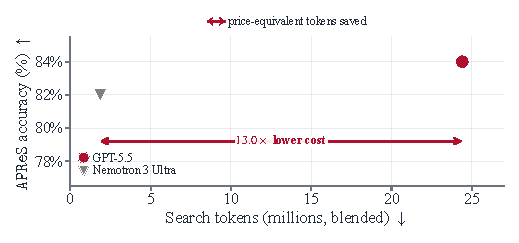
\includegraphics[width=\linewidth]{figures/fig_nemotron_cost_shift.pdf}
\caption{\textbf{\nemotronultra task-agent calls approach the \gptlow-only run at $\approx$\textbf{13.0}$\boldsymbol{\times}$ lower search-token cost.} On the held-out \apres split, final \gptlow evaluation shows that the \nemotronultra-discovered harness approaches the performance of our \gptlow-only harness. Since raw tokens are not directly comparable, we report \gptlow-price-equivalent blended tokens based on the best available pricing at the time of writing. Expansion calls are charged the same as in \gptlow-only runs~(\cref{app:domain-protocols}).}
\label{fig:nemotron-cost-shift}
\end{wrapfigure}

\noindent\textbf{Price-equivalent accounting.}~~As shown in \cref{fig:nemotron-cost-shift}, replacing \gptlow with \nemotronultra as the task agent reduces search-token costs by $\approx$\textbf{13.0}$\boldsymbol{\times}$ while approaching the \gptlow-only run's accuracy under the same final evaluation. We expect this benefit to be domain-specific, depending on whether the cheaper task agent provides an informative signal. If the task-agent foundation model is insufficiently capable for a domain, for example constructing novel proofs, it may increase search costs because different meta-agent expansions become hard to distinguish in quality.
\vspace{-0.17cm}
\takeawaybox[Cost ablation:]{Empirically, the primary cost driver in \theourmethod search is evaluation, not expansion. In paper review, routing search-time task-agent calls through a more efficient foundation model substantially reduces search cost with tolerable final-performance loss; this trade-off remains to be investigated for other domains.}
\clearpage